%!TEX root = ../../thirdYearReport.tex


\newcommand{\EQ}{\!\!\!=\!\!\!}

\newcommand{\Bp}{\mathbf{p}}
\newcommand{\Br}{\mathbf{r}}
\newcommand{\Bf}{\mathbf{f}}
\newcommand{\BJ}{\mathbf{J}}
\newcommand{\Bv}{\mathbf{v}}
\newcommand{\BI}{\mathbf{I}}
\newcommand{\BR}{\mathbf{R}}
\newcommand{\BK}{\mathbf{K}}
\newcommand{\BD}{\mathbf{D}}
\newcommand{\BA}{\mathbf{A}}
\newcommand{\Bb}{\mathbf{b}}
\newcommand{\BM}{\mathbf{M}}
\newcommand{\BC}{\mathbf{C}}
\newcommand{\Bg}{\mathbf{g}}
\newcommand{\BS}{\mathbf{S}}
\newcommand{\Bzero}{\mathbf{0}}
\newcommand{\BN}{\mathbf{N}}
\newcommand{\Bh}{\mathbf{h}}
\newcommand{\BW}{\mathbf{W}}
\newcommand{\Bq}{\mathbf{q}}
\newcommand{\BF}{\mathbf{F}}
\newcommand{\Bn}{\mathbf{n}}
\newcommand{\BZ}{\mathbf{Z}}
\newcommand{\BB}{\mathbf{B}}
\newcommand{\Bc}{\mathbf{c}}

\newcommand{\Bomega}{\boldsymbol{\omega}}
\newcommand{\Btau}{\boldsymbol{\tau}}
\newcommand{\Balpha}{\boldsymbol{\alpha}}
\newcommand{\Bbeta}{\boldsymbol{\beta}}



\paragraph{Work package 1 progress}

\subparagraph{Software architecture design and evaluation of available
  open-source software pertinent to the scope of the project. (T1.1)}

The goal of T1.1 was to agree on a specific software architecture with
associated software tools whose specifications, dependencies and
interconnections meet the requirements and needs for achieving the goals of
the project.  The software, which is called \texttt{codyco-superbuild}, has
been available via github on
\texttt{https://github.com/robotology/codyco-superbuild} since the second year
of the project.  Details about the modules of the software are available in
deliverables D1.1, D1.2 and D1.3.

\subparagraph{Simulator for whole-body motion with contacts (T1.2)}

The CoDyCo project requires a modular, component-based dynamics simulation
software providing numerically stable, computationally efficient and
physically consistent simulations of whole-body virtual human(oid) systems in
contact with rigid or soft environments.  To this end, in year one, a new iCub
simulator was released and documented as part of deliverable D1.1.


\subparagraph{Control library for flexible specification of task space
  dynamics of floating base manipulators. (T1.3)}

%UPMC has recently developed OCRA ``Optimization-based Control for Robotics
%Applications'' which is available from
%\url{https://github.com/ocra-recipes/ocra-recipes}.  This has been tested on
%the iCubParis02 and the KUKA LWR.

UPMC has developed OCRA which stands for Optimization-based Control for Robotics Applications. OCRA is a set of tools which facilitates the development of optimization-based controllers for robots. At its core there is \href{https://github.com/ocra-recipes/ocra-recipes}{ocra-recipes}, a group of platform independent libraries which can be used to quickly develop optimization based controllers for any robot. Hierarchical, weighted, and hybrid controller schemes can easily be implemented using the \href{https://github.com/ocra-recipes/ocra-recipes}{ocra-recipes} libraries. The generic interfaces provided by OCRA allow different robots to use the exact same controllers. Examples of such implementations can be found for the humanoid robot iCub (\href{https://github.com/ocra-recipes/ocra-wbi-plugins}{ocra-wbi-plugins}), and the 7 DoF Kuka LWR (\href{https://github.com/kuka-isir/ocra-kdl}{ocra-kdl}). OCRA. also allows users to specify high-level objectives via tasks. These tasks provide an intuitive way of generating complex behaviours and can be specified in XML format.

%Tasks can be specified in XML, use hierarchical, weighted or hybrid QP control
%and use QuadProg++ or qpOases as your solver. More to come soon.


\subparagraph{System dynamics estimation software. Extension to
environmental compliance estimation (T1.4)}

As a part of this task, UB and TUD developed a framework in order to estimate
the parameters of compliant contacts between the robot and its environment.
Using this framework, we can predict contact forces in the next instant.
Assume that the body which is in contact with a soft surface is labeled with
$B_c$.  We characterize the contact surface of $B_c$ by $m$ fictitious contact
points on this body.  Let $\Bp_i$ denote the position of the i$^{th}$ contact
point ($i=1,2,\ldots,m$) in the world frame.  Therefore,
%
\begin{equation}
  \Bp_i = \Bp + \BR \Br_i \, ,
\end{equation}
%
where $\Bp$ is the position of the origin of the local frame of $B_c$ with
respect to the world frame, $\BR$ is the rotation matrix of $B_c$ with respect
to the world frame and $\Br_i$ is the position of i$^{th}$ contact point in
the local frame of $B_c$.  So
%
\begin{equation}
  \dot{\Bp}_i = \dot{\Bp} + \dot{\BR} \Br_i = \dot{\Bp} - (\BR\Br_i)^{\wedge}
  \Bomega = [ \BI_{3 \times 3} \; \; {}-(\BR\Br_i)^{\wedge} ] \BJ_s \Bv \, ,
  \label{pidot}
\end{equation}
%
where $\BJ_s$ is the Jacobian of the bodies in contact with soft surfaces,
$\Bomega$ is the angular velocity of $B_c$ and $()^{\wedge}$ represents the
skew symmetric matrix.  We also have
%
\begin{equation}
  \ddot{\Bp}_i = \ddot{\Bp} + \ddot{\BR} \Br_i = \ddot{\Bp} - (\BR
  \Br_i)^{\wedge} \dot{\Bomega} + (\Bomega)^{\wedge} (\Bomega)^{\wedge} \BR
  \Br_i = [ \BI_{3 \times 3} \; \; {}-(\BR \Br_i)^{\wedge}] (\dot{\BJ}_s \Bv +
  \BJ_s \dot{\Bv}) + (\Bomega)^{\wedge} (\Bomega)^{\wedge} \BR \Br_i \, .
  \label{piddot}
\end{equation}
%

According to contact mechanics \cite{Johnson77} and its applications in
robotics \cite{Azad&Featherstone10, Azad&Featherstone14a, Hunt&Crossley75,
  Marhefka&Orin99}, there is a non-linear relationship between compliant
contact force and the deformation and the rate of the deformation of the
surface.  However, in order to simplify the model, we assume a locally linear
relationship between the change of the contact force and the change of the
deformation and its rate.  Based on this assumption, we can write
%
\begin{equation}
  \delta \Bf_i = \BK \delta \Bp_i + \BD \delta \dot{\Bp}_i \, ,
\end{equation}
%
where $\delta \Bf_i$ and $\delta \Bp_i$ are the changes of the contact force
and the deformation at the i$^{th}$ contact point, respectively, and $\BK$ and
$\BD$ are $3 \times 3$ matrices of the coefficients of stiffness and damping,
respectively.  By using a linear integration method, we can estimate $\delta
\Bp_i$ and $\delta \dot{\Bp}_i$ as
%
\begin{equation}
  \delta \Bp_i = \dot{\Bp}_i \delta t + \frac{1}{2} \ddot{\Bp}_i \delta t^2 \,
  ,
  \label{deltapi}
\end{equation}
%
and
%
\begin{equation}
  \delta \dot{\Bp}_i = \ddot{\Bp}_i \delta t \, ,
  \label{deltapidot}
\end{equation}
%
where $\delta t$ is the sampling time.  Hence, by substituting (\ref{pidot})
and (\ref{piddot}) into (\ref{deltapi}) and (\ref{deltapidot}), we will have
%
\begin{equation}
  \delta \Bf_i = \BA_i \dot{\Bv} + \Bb_i \, ,
\end{equation}
%
where
%
%
\begin{equation}
  \BA_i = \frac{1}{2} \delta t^2 [\BK \; \; -\BK(\BR \Br_i)^{\wedge}] \BJ_s +
  \delta t [\BD \; \; - \BD(\BR \Br_i)^{\wedge}] \BJ_s \, ,
\end{equation}
%
and
%
\begin{eqnarray}
  \nonumber \Bb_i & \EQ & \delta t [\BK \; \; -\BK(\BR \Br_i)^{\wedge}] \BJ_s
  \Bv + \frac{1}{2} \delta t^2 [\BK \; \; -\BK(\BR \Br_i)^{\wedge}]
  \dot{\BJ}_s \Bv\\ & & + \frac{1}{2} \delta t^2 \BK (\Bomega)^{\wedge}
  (\Bomega)^{\wedge} \BR \Br_i + \delta t [\BD \; \; -\BD(\BR \Br_i)^{\wedge}]
  \dot{\BJ}_s \Bv + \delta t \BD (\Bomega)^{\wedge} (\Bomega)^{\wedge} \BR
  \Br_i \, .
\end{eqnarray}
%
Also for the moment of the contact forces we have
%
\begin{equation}
  \delta \Bn_i = (\BR \Br_i)^{\wedge} \delta \Bf_i \, .
\end{equation}
%
Therefore, total change of the force vector for $B_c$ will be
%
\begin{equation}
  \delta \Bf_s =
  \begin{bmatrix}
    \sum_{i=1}^m \BA_i \dot{\Bv} + \sum_{i=1}^m \Bb_i\\
    \\
    \sum_{i=1}^m (\BR \Br_i)^{\wedge} \BA_i \dot{\Bv} + \sum_{i=1}^m \Bb_i
  \end{bmatrix}
  =
  \begin{bmatrix}
    \BA_f \\
    \\
    \BA_n
  \end{bmatrix}
  \dot{\Bv} +
  \begin{bmatrix}
    \Bb_f \\
    \\
    \Bb_n
  \end{bmatrix}
  = \BA \dot{\Bv} + \Bb \, .
\end{equation}
%
Hence, the estimated (for the next instant) 6D force-torque vector of the
contact force of $B_c$ will be
%
\begin{equation}
  \hat{\Bf}_s = \Bf_s + \delta \Bf_s = \BA \dot{\Bv} + \Bb + \Bf_s \, ,
\end{equation}
%
which is a function of contact parameters ($\BK$ and $\BD$), current force
(read from F/T sensors) and joint accelerations ($\dot{\Bv}$).  Note that for
the constraints on the soft contact force (unilaterality and friction cone),
$\hat{\Bf}_s$ has to be expressed in the local frame of $B_c$ as $\hat{\BF}_s
= \BR^T \hat{\Bf}_s$.

In order to estimate the contact parameters ($\BK$ and $\BD$), we use locally
weighted projection regression (LWPR) algorithm.  This algorithm gives us a
locally linear model for a non-linear function which suits our application.
The outcome of this algorithm will be $\BK$ and $\BD$ at each time instant
based on the previous values of the contact force and the position and
velocity of the contact point.  Therefore, we can compute the (estimation of
the) contact force in the next instant.  Implementation of this algorithm is
available from \url{https://github. com/azadm/LWR_for_ContactParams.git}.  To
verify this algorithm, TUD performed a few experiments on iCub robot standing
on soft surfaces.  During those experiments, the robot was standing on two
different surfaces (transparent plastic and white foam) while balancing
controller was running on the robot.  The upper body of the robot was
perturbed and data from all sensors were collected in order to calculate the
movements of the contact points and also the contact forces.  By feeding these
values into our LWPR algorithm, we estimated the contact force and compared
with the actual data from F/T sensors.  The results are acceptable and show
the consistency of the LWPR estimation algorithm.  For example,
Fig~\ref{force_estimate} shows the match between actual and estimated change
of the contact force in the vertical direction while the robot's right foot is
on a soft surface (i.e. white foam).
%
\begin{figure}
  \centering
  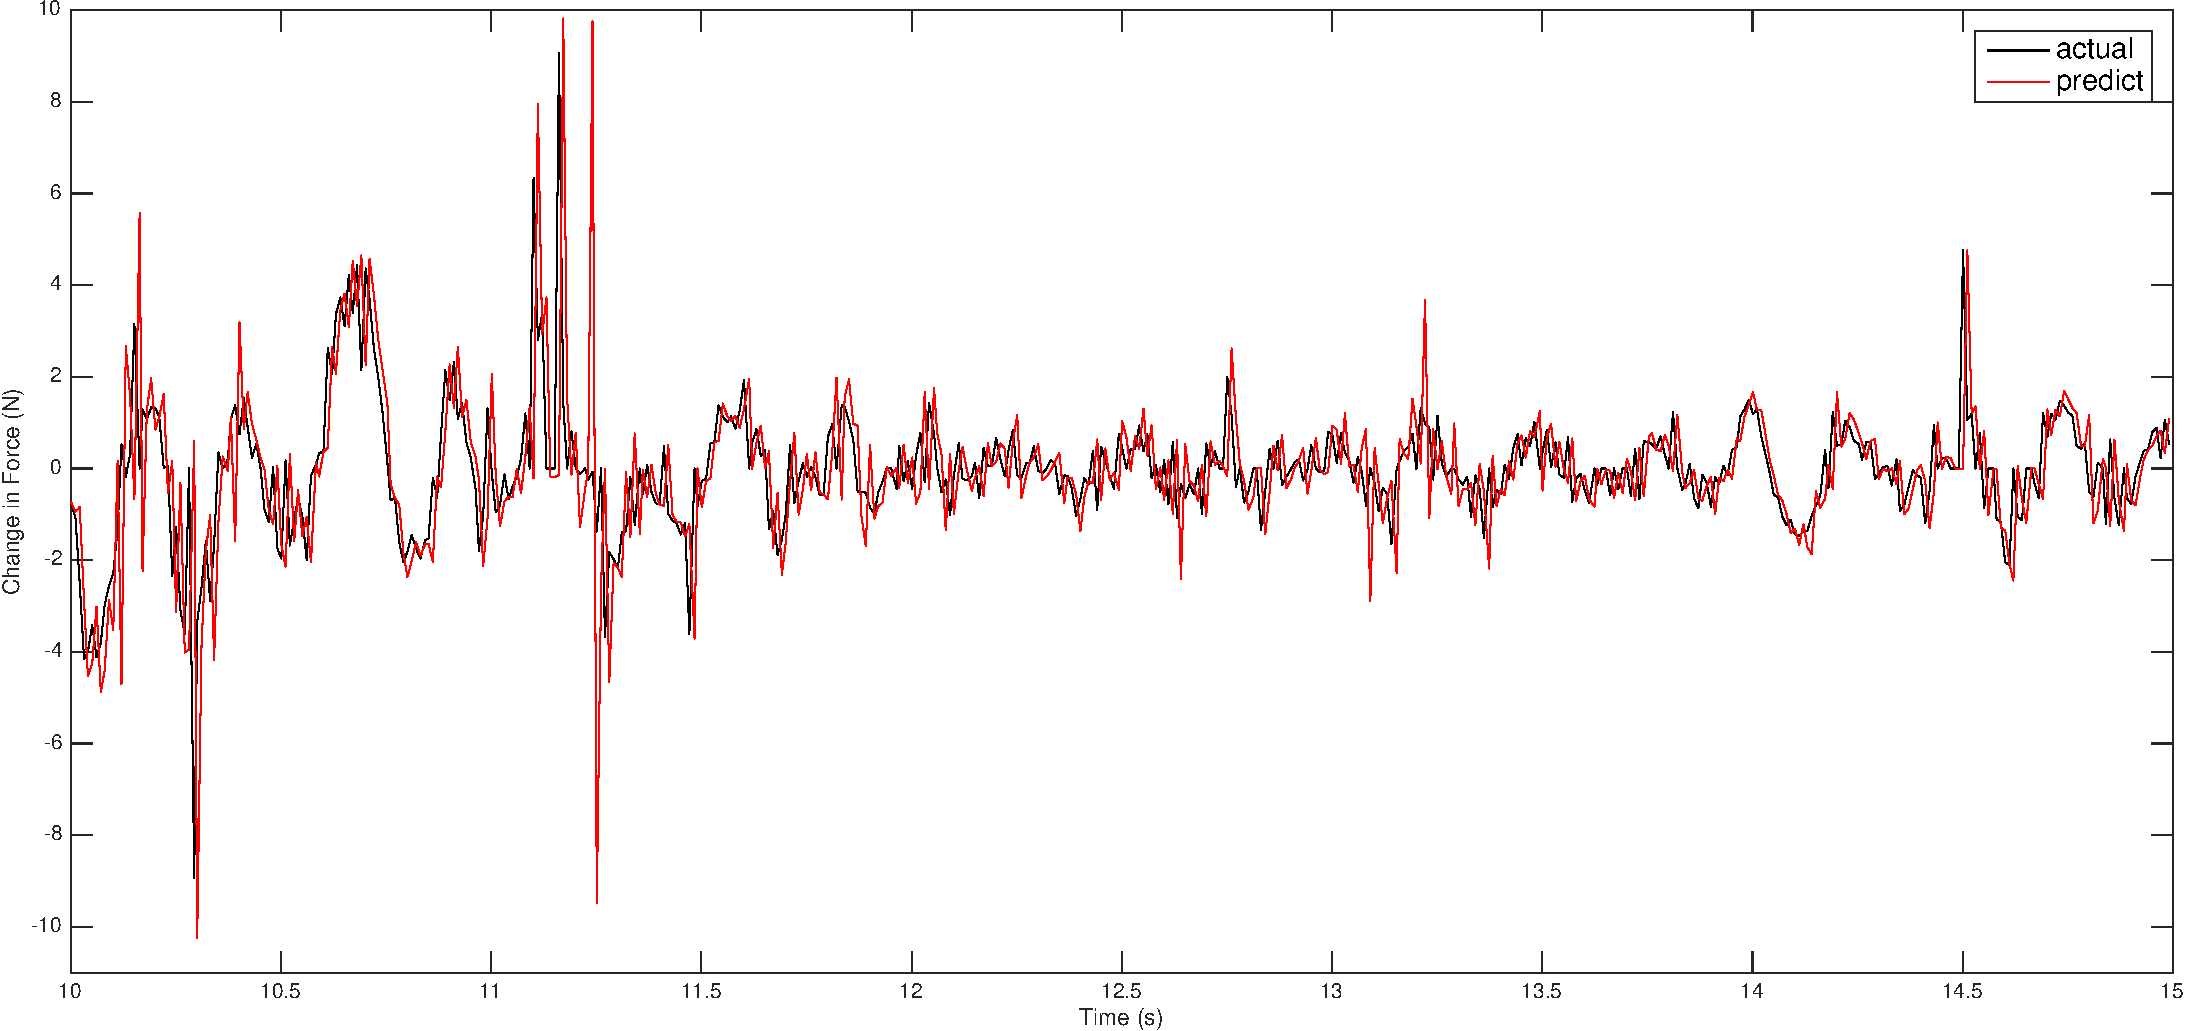
\includegraphics[scale=0.4]{images/force_estimate.pdf}
  \caption{Change of contact force in the vertical direction.  The right foot
    of the iCub is placed on a white foam.}
  \label{force_estimate}
\end{figure}


\subparagraph{Extension and enhancement of the iDyn library. (T1.5)}
\label{sec:T15}

\emph{IIT to provide input about floating base estimation.}








